\documentclass[tikz,border=1pt]{standalone}
\usepackage{tikz}
\usetikzlibrary{arrows.meta,positioning}
\definecolor{ink}{HTML}{1A2433}
\definecolor{steel}{HTML}{21506F}
\definecolor{loadedblue}{HTML}{0072B2}
\definecolor{emptyorange}{HTML}{E69F00}
\definecolor{transfergreen}{HTML}{009E73}
\definecolor{selectamber}{HTML}{FFC107}
\definecolor{pale}{HTML}{F2F6FA}
\definecolor{paleblue}{HTML}{E7F2FB}
\begin{document}
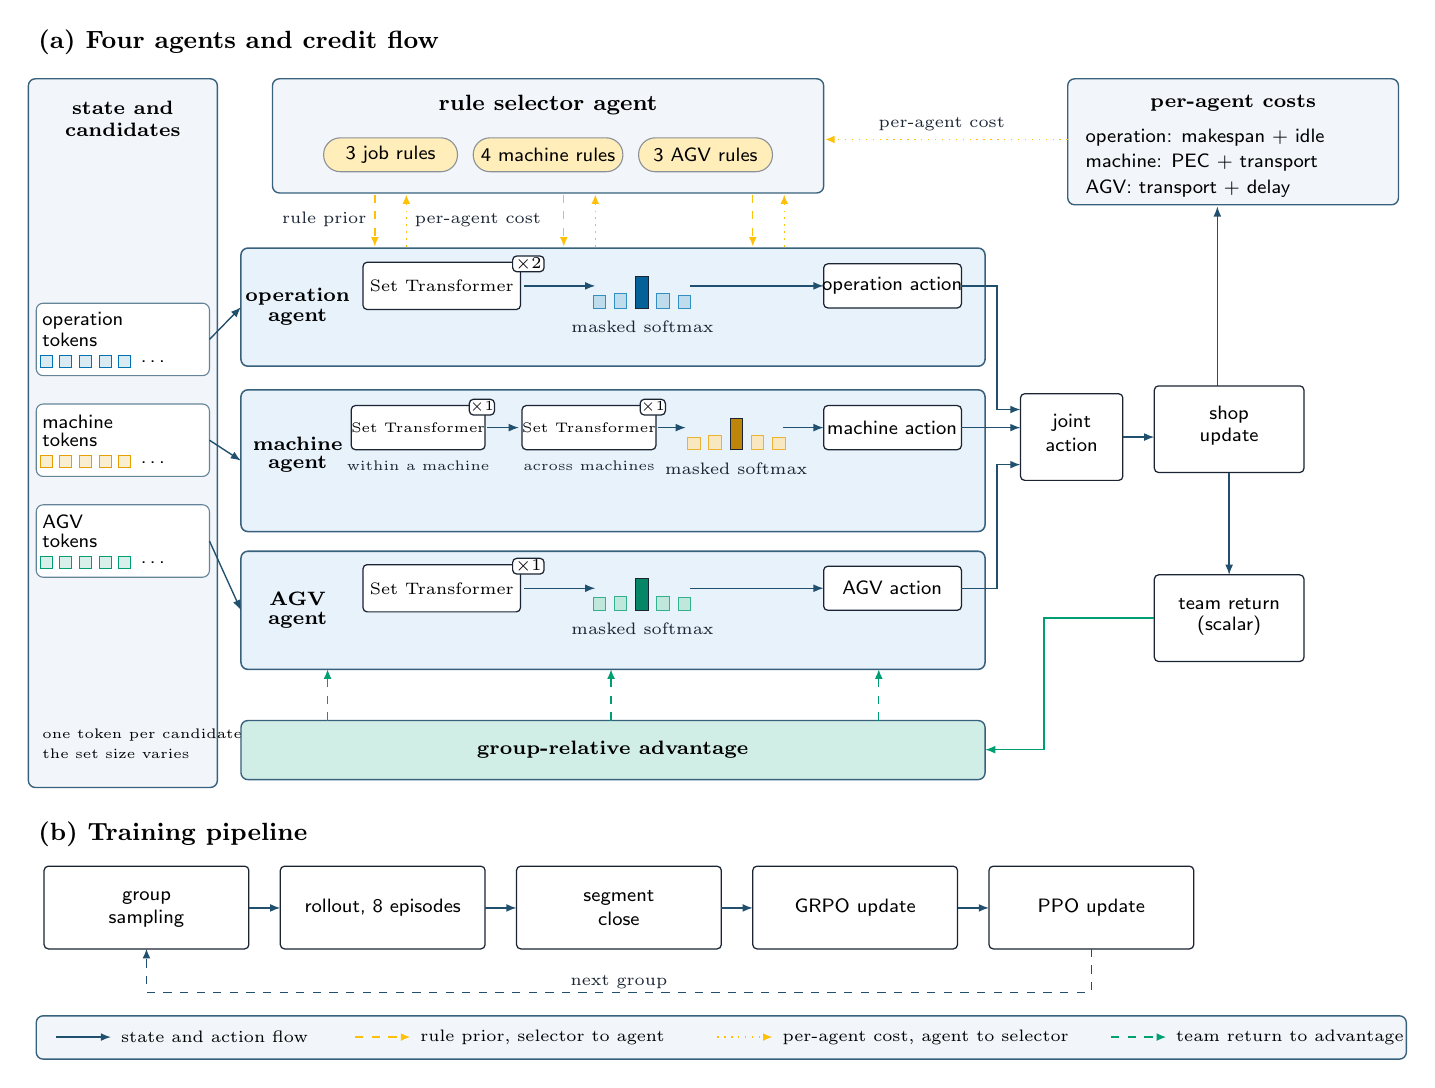
\begin{tikzpicture}[y=-1cm,x=1cm,font=\sffamily\fontsize{7.2}{8.6}\selectfont,
  every node/.style={inner sep=0.6pt},
  card/.style={draw=steel!90,line width=0.5pt,fill=pale,rounded corners=2.5pt},
  tokbox/.style={draw=steel!70,line width=0.4pt,fill=white,rounded corners=2.5pt},
  lane/.style={draw=steel!90,line width=0.55pt,fill=paleblue,rounded corners=2.5pt},
  mod/.style={draw=ink,line width=0.45pt,fill=white,rounded corners=1.5pt},
  pill/.style={draw=ink!50,line width=0.4pt,fill=selectamber!28!white,rounded corners=6pt},
  flow/.style={-{Latex[length=1.3mm,width=1.0mm]},line width=0.5pt,draw=steel},
  selectdash/.style={-{Latex[length=1.2mm,width=1.0mm]},line width=0.5pt,draw=selectamber,dashed},
  selectdot/.style={-{Latex[length=1.2mm,width=1.0mm]},line width=0.5pt,draw=selectamber,dotted},
  greenflow/.style={-{Latex[length=1.3mm,width=1.0mm]},line width=0.55pt,draw=transfergreen},
  greendash/.style={-{Latex[length=1.2mm,width=1.0mm]},line width=0.5pt,draw=transfergreen,dashed},
  loop/.style={-{Latex[length=1.2mm,width=1.0mm]},line width=0.45pt,draw=steel,dashed},
  title/.style={anchor=west,font=\bfseries\fontsize{8.6}{10.2}\selectfont},
  lab/.style={text=ink},
  small/.style={font=\fontsize{5.8}{6.8}\selectfont,text=ink},
]

% ================= (a) =================
\node[title] at (0.30,0.48) {(a) Four agents and credit flow};

% selector card
\draw[card] (3.30,0.95) rectangle (10.30,2.40);
\node[font=\bfseries\fontsize{7.6}{9.0}\selectfont] at (6.80,1.28) {rule selector agent};
\draw[pill] (3.95,1.70) rectangle (5.65,2.13);
\node at (4.80,1.915) {3 job rules};
\draw[pill] (5.85,1.70) rectangle (7.75,2.13);
\node at (6.80,1.915) {4 machine rules};
\draw[pill] (7.95,1.70) rectangle (9.65,2.13);
\node at (8.80,1.915) {3 AGV rules};

% per-agent costs card
\draw[card] (13.40,0.95) rectangle (17.60,2.55);
\node[font=\bfseries\fontsize{7.4}{8.8}\selectfont] at (15.50,1.26) {per-agent costs};
\node[anchor=west] at (13.60,1.70) {operation: makespan + idle};
\node[anchor=west] at (13.60,2.02) {machine: PEC + transport};
\node[anchor=west] at (13.60,2.34) {AGV: transport + delay};

% state card
\draw[card] (0.20,0.95) rectangle (2.60,9.95);
\node[font=\bfseries\fontsize{7.4}{8.8}\selectfont] at (1.40,1.32) {state and};
\node[font=\bfseries\fontsize{7.4}{8.8}\selectfont] at (1.40,1.60) {candidates};
\draw[tokbox] (0.30,3.80) rectangle (2.50,4.72);
\draw[tokbox] (0.30,5.08) rectangle (2.50,6.00);
\draw[tokbox] (0.30,6.36) rectangle (2.50,7.28);
\node[anchor=west] at (0.35,4.02) {operation};
\node[anchor=west] at (0.35,4.26) {tokens};
\foreach \k in {0,1,2,3,4} {
  \fill[loadedblue!15!white,draw=loadedblue,line width=0.35pt] (0.35+0.25*\k,4.46) rectangle (0.50+0.25*\k,4.61);
}
\node[anchor=west] at (1.60,4.54) {\ldots};
\node[anchor=west] at (0.35,5.30) {machine};
\node[anchor=west] at (0.35,5.54) {tokens};
\foreach \k in {0,1,2,3,4} {
  \fill[emptyorange!18!white,draw=emptyorange,line width=0.35pt] (0.35+0.25*\k,5.74) rectangle (0.50+0.25*\k,5.89);
}
\node[anchor=west] at (1.60,5.82) {\ldots};
\node[anchor=west] at (0.35,6.58) {AGV};
\node[anchor=west] at (0.35,6.82) {tokens};
\foreach \k in {0,1,2,3,4} {
  \fill[transfergreen!15!white,draw=transfergreen,line width=0.35pt] (0.35+0.25*\k,7.02) rectangle (0.50+0.25*\k,7.17);
}
\node[anchor=west] at (1.60,7.10) {\ldots};
\node[anchor=west,font=\fontsize{5.0}{6.0}\selectfont] at (0.35,9.28) {one token per candidate;};
\node[anchor=west,font=\fontsize{5.0}{6.0}\selectfont] at (0.35,9.52) {the set size varies};

% lanes
\draw[lane] (2.90,3.10) rectangle (12.35,4.60);
\draw[lane] (2.90,4.90) rectangle (12.35,6.70);
\draw[lane] (2.90,6.95) rectangle (12.35,8.45);

% operation lane
\node[font=\bfseries\fontsize{7.4}{8.8}\selectfont] at (3.62,3.72) {operation};
\node[font=\bfseries\fontsize{7.4}{8.8}\selectfont] at (3.62,3.98) {agent};
\draw[mod] (4.45,3.28) rectangle (6.45,3.88);
\node[font=\fontsize{6.2}{7.4}\selectfont] at (5.45,3.58) {Set Transformer};
\draw[mod] (6.35,3.20) rectangle (6.75,3.40);
\node[font=\fontsize{5.6}{6.4}\selectfont] at (6.55,3.30) {$\times2$};
\draw[flow] (6.50,3.58) -- (7.40,3.58);
\foreach \x/\h in {7.45/0.16,7.72/0.18,7.99/0.40,8.26/0.18,8.53/0.16} {
  \fill[loadedblue!25!white,draw=loadedblue!80,line width=0.3pt] (\x-0.08,3.86) rectangle (\x+0.08,3.86-\h);
}
\fill[loadedblue!80!ink,draw=ink,line width=0.3pt] (7.91,3.86) rectangle (8.07,3.46);
\node[small] at (8.00,4.10) {masked softmax};
\draw[flow] (8.60,3.58) -- (10.30,3.58);
\draw[mod] (10.30,3.30) rectangle (12.05,3.86);
\node at (11.17,3.58) {operation action};

% machine lane
\node[font=\bfseries\fontsize{7.4}{8.8}\selectfont] at (3.62,5.58) {machine};
\node[font=\bfseries\fontsize{7.4}{8.8}\selectfont] at (3.62,5.84) {agent};
\draw[mod] (4.30,5.10) rectangle (6.00,5.66);
\node[font=\fontsize{5.0}{6.0}\selectfont] at (5.15,5.38) {Set Transformer};
\draw[mod] (5.80,5.02) rectangle (6.12,5.22);
\node[font=\fontsize{5.0}{5.8}\selectfont] at (5.96,5.12) {$\times1$};
\node[font=\fontsize{4.8}{5.8}\selectfont,text=ink] at (5.15,5.86) {within a machine};
\draw[flow] (6.03,5.38) -- (6.43,5.38);
\draw[mod] (6.47,5.10) rectangle (8.17,5.66);
\node[font=\fontsize{5.0}{6.0}\selectfont] at (7.32,5.38) {Set Transformer};
\draw[mod] (7.97,5.02) rectangle (8.29,5.22);
\node[font=\fontsize{5.0}{5.8}\selectfont] at (8.13,5.12) {$\times1$};
\node[font=\fontsize{4.8}{5.8}\selectfont,text=ink] at (7.32,5.86) {across machines};
\draw[flow] (8.20,5.38) -- (8.55,5.38);
\foreach \x/\h in {8.65/0.16,8.92/0.18,9.19/0.40,9.46/0.18,9.73/0.16} {
  \fill[emptyorange!25!white,draw=emptyorange!80,line width=0.3pt] (\x-0.08,5.66) rectangle (\x+0.08,5.66-\h);
}
\fill[emptyorange!80!ink,draw=ink,line width=0.3pt] (9.11,5.66) rectangle (9.27,5.26);
\node[small] at (9.19,5.90) {masked softmax};
\draw[flow] (9.78,5.38) -- (10.30,5.38);
\draw[mod] (10.30,5.10) rectangle (12.05,5.66);
\node at (11.17,5.38) {machine action};

% AGV lane
\node[font=\bfseries\fontsize{7.4}{8.8}\selectfont] at (3.62,7.56) {AGV};
\node[font=\bfseries\fontsize{7.4}{8.8}\selectfont] at (3.62,7.82) {agent};
\draw[mod] (4.45,7.12) rectangle (6.45,7.72);
\node[font=\fontsize{6.2}{7.4}\selectfont] at (5.45,7.42) {Set Transformer};
\draw[mod] (6.35,7.04) rectangle (6.75,7.24);
\node[font=\fontsize{5.6}{6.4}\selectfont] at (6.55,7.14) {$\times1$};
\draw[flow] (6.50,7.42) -- (7.40,7.42);
\foreach \x/\h in {7.45/0.16,7.72/0.18,7.99/0.40,8.26/0.18,8.53/0.16} {
  \fill[transfergreen!25!white,draw=transfergreen!80,line width=0.3pt] (\x-0.08,7.70) rectangle (\x+0.08,7.70-\h);
}
\fill[transfergreen!80!ink,draw=ink,line width=0.3pt] (7.91,7.70) rectangle (8.07,7.30);
\node[small] at (8.00,7.94) {masked softmax};
\draw[flow] (8.60,7.42) -- (10.30,7.42);
\draw[mod] (10.30,7.14) rectangle (12.05,7.70);
\node at (11.17,7.42) {AGV action};

% state to lanes
\draw[flow] (2.50,4.26) -- (2.90,3.85);
\draw[flow] (2.50,5.54) -- (2.90,5.80);
\draw[flow] (2.50,6.82) -- (2.90,7.70);

% rule prior trunk (left)
\foreach \x in {4.60,7.00,9.40} { \draw[selectdash] (\x,2.42) -- (\x,3.08); }
\foreach \x in {5.00,7.40,9.80} { \draw[selectdot] (\x,3.08) -- (\x,2.42); }
\node[small] at (4.52,2.74) [anchor=east] {rule prior};
\node[small] at (5.08,2.74) [anchor=west] {per-agent cost};

% per-agent costs: shop -> card, card -> selector
\draw[selectdot] (13.40,1.72) -- (10.32,1.72);
\node[small] at (11.80,1.52) {per-agent cost};
\draw[flow] (15.30,4.85) -- (15.30,2.57);

% joint action
\draw[mod] (12.80,4.95) rectangle (14.10,6.05);
\node at (13.45,5.32) {joint};
\node at (13.45,5.60) {action};
\draw[flow] (12.05,3.58) -- (12.50,3.58) -- (12.50,5.15) -- (12.80,5.15);
\draw[flow] (12.05,5.38) -- (12.80,5.38);
\draw[flow] (12.05,7.42) -- (12.50,7.42) -- (12.50,5.85) -- (12.80,5.85);

% shop update, team return, advantage
\draw[mod] (14.50,4.85) rectangle (16.40,5.95);
\node at (15.45,5.22) {shop};
\node at (15.45,5.50) {update};
\draw[flow] (14.10,5.50) -- (14.50,5.50);
\draw[mod] (14.50,7.25) rectangle (16.40,8.35);
\node at (15.45,7.62) {team return};
\node at (15.45,7.90) {(scalar)};
\draw[flow] (15.45,5.95) -- (15.45,7.25);
\draw[card,fill=transfergreen!18!white] (2.90,9.10) rectangle (12.35,9.85);
\node[font=\bfseries\fontsize{7.4}{8.8}\selectfont] at (7.62,9.47) {group-relative advantage};
\draw[greenflow] (14.50,7.80) -- (13.10,7.80) -- (13.10,9.47) -- (12.35,9.47);
\draw[greendash] (4.00,9.10) -- (4.00,8.45);
\draw[greendash] (7.60,9.10) -- (7.60,8.45);
\draw[greendash] (11.00,9.10) -- (11.00,8.45);

% ================= (b) =================
\node[title] at (0.30,10.55) {(b) Training pipeline};
\draw[mod] (0.40,10.95) rectangle (3.00,12.00);
\node at (1.70,11.35) {group};
\node at (1.70,11.62) {sampling};
\draw[mod] (3.40,10.95) rectangle (6.00,12.00);
\node at (4.70,11.48) {rollout, 8 episodes};
\draw[mod] (6.40,10.95) rectangle (9.00,12.00);
\node at (7.70,11.35) {segment};
\node at (7.70,11.62) {close};
\draw[mod] (9.40,10.95) rectangle (12.00,12.00);
\node at (10.70,11.48) {GRPO update};
\draw[mod] (12.40,10.95) rectangle (15.00,12.00);
\node at (13.70,11.48) {PPO update};
\draw[flow] (3.00,11.48) -- (3.40,11.48);
\draw[flow] (6.00,11.48) -- (6.40,11.48);
\draw[flow] (9.00,11.48) -- (9.40,11.48);
\draw[flow] (12.00,11.48) -- (12.40,11.48);
\draw[loop] (13.70,12.00) -- (13.70,12.55) -- (1.70,12.55) -- (1.70,12.00);
\node[small] at (7.70,12.42) {next group};

% ================= legend =================
\draw[card] (0.30,12.85) rectangle (17.70,13.40);
\draw[flow] (0.55,13.12) -- (1.25,13.12);
\node[anchor=west,font=\fontsize{6.0}{7.0}\selectfont] at (1.35,13.12) {state and action flow};
\draw[selectdash] (4.35,13.12) -- (5.05,13.12);
\node[anchor=west,font=\fontsize{6.0}{7.0}\selectfont] at (5.15,13.12) {rule prior, selector to agent};
\draw[selectdot] (8.95,13.12) -- (9.65,13.12);
\node[anchor=west,font=\fontsize{6.0}{7.0}\selectfont] at (9.75,13.12) {per-agent cost, agent to selector};
\draw[greendash] (13.95,13.12) -- (14.65,13.12);
\node[anchor=west,font=\fontsize{6.0}{7.0}\selectfont] at (14.75,13.12) {team return to advantage};

\end{tikzpicture}
\end{document}